%%%%%%%%%%%%%%%%%%%%% {{{
%%Options for presentations (in-class) and handouts (e.g. print).
% \documentclass[pdf,9pt]{beamer}
\documentclass[pdf,9pt]{beamer}


%%%%%%%%%%%%%%%%%%%%%%
%Change this for different slides so it appears in bar
\usepackage{authoraftertitle}
\author{}

\date{Chapter 5. Vector Space $\RR^n$\\ \S 5-1. Subspaces and Spanning}

%%%%%%%%%%%%%%%%%%%%%%
%% Upload common style file
\usepackage{LyryxLAWASlidesStyle}

\begin{document}

%%%%%%%%%%%%%%%%%%%%%%%
%% Title Page and Copyright Common to All Slides

%Title Page
\input frontmatter/titlepage.tex

%LOTS Page
\input frontmatter/lyryxopentexts.tex

%Copyright Page
\input frontmatter/copyright.tex

%%%%%%%%%%%%%%%%%%%%%%%%% }}}
%-------------- start slide -------------------------------%{{{ 2
\begin{frame}[fragile]
   \tableofcontents
\end{frame}
%-------------- end slide -------------------------------%}}}
\section[\textcolor{yellow}{}]{\textcolor{yellow}{Subspaces of $\RR^n$}}
%-------------- start slide -------------------------------%{{{ 3
\frame{
\frametitle{Subspaces of $\R^n$}
\pause
\begin{definitions}
\begin{enumerate}
    \item $\RR$ denotes the set of \alert{real} numbers, and is an example of a
	set of \alert{scalars}.

    \item $\RR^n$ is the set of all $n$-tuples of real numbers, i.e.,
    \[ \RR^n=\left\{ (x_1, x_2, \ldots, x_n) ~|~ x_i\in\RR, 1\leq i\leq n
    \right\}.\]

    \item The \textcolor{red}{vector space} $\RR^n$ consists of the set $\RR^n$
	written as \textcolor{red}{column matrices}, along with the (matrix)
	operations of addition and scalar multiplication.  Unless stated
	otherwise, $\RR^n$ means the vector space $\RR^n$.
\end{enumerate}
\end{definitions}
\vfill
\pause

\begin{remark}
    $\RR^n$ is a concrete example of the abstract vector space will be studied in the next chapter.
\end{remark}
}
%-------------- end slide -------------------------------%}}}
%-------------- start slide -------------------------------%{{{ 4
\frame{
\begin{emptytitle}
    A vectors is denoted by a lower case letter with an arrow
    written over it; for example,
    $\vec{u}$, $\vec{v}$, and $\vec{x}$ denote vectors.\\[1em]
    \pause

    Another example: $\vec{u}=\left[ \begin{array}{r} -2 \\3\\ 0.7 \\ 5\\ \pi \end{array}\right]$
    is a vector in $\RR^5$, written ${\vec u}\in\RR^5$.\\[1em]

    \pause
    To save space on the page, the same vector $\vec u$
    may be written instead as a row matrix by taking the transpose of
    the column:
    \[ \vec{u}=\left[\begin{array}{ccccc}
    -2, & 3, & 0.7, & 5, & \pi \end{array}\right]^T.\]
\end{emptytitle}
}
%-------------- end slide -------------------------------%}}}
%-------------- start slide -------------------------------%{{{ 5
\frame{
    \begin{emptytitle}
	We are interested in {\em nice} subsets of  $\RR^n$, defined as follows.
    \end{emptytitle}
\pause
\begin{definition}[Subspaces]
    A subset $U$ of $\RR^n$ is a \alert{subspace} of $\RR^n$ if
    \begin{enumerate}
	\item[S1.] The zero vector of $\RR^n$, $\vec{0}_n$, is in $U$;
	\item[S2.] $U$ is closed under addition, i.e., for all $\vec{u},\vec{w}\in U$, $\vec{u}+\vec{w}\in U$;
	\item[S3.] $U$ is closed under scalar multiplication, i.e., for all $\vec{u}\in U$ and $k\in\RR$, $k\vec{u}\in U$.
    \end{enumerate}
    \pause
    Both subset $U=\left\{ \vec{0}_n\right\}$ and $R^n$ itself are subspaces of
    $\RR^n$.
    Any other subspace of $\RR^n$ is called a \alert{proper} subspace of $\RR^n$.
\end{definition}
\vfill

\pause
\begin{block}{Notation}
If $U$ is a subset of $\RR^n$, we write $U\subseteq\RR^n$.
\end{block}
}
%-------------- end slide -------------------------------%}}}
%-------------- start slide -------------------------------%{{{ 6
\begin{frame}[fragile]
    \vspace{-7em}
    \begin{picture}(2,2)
	\put(1,-1){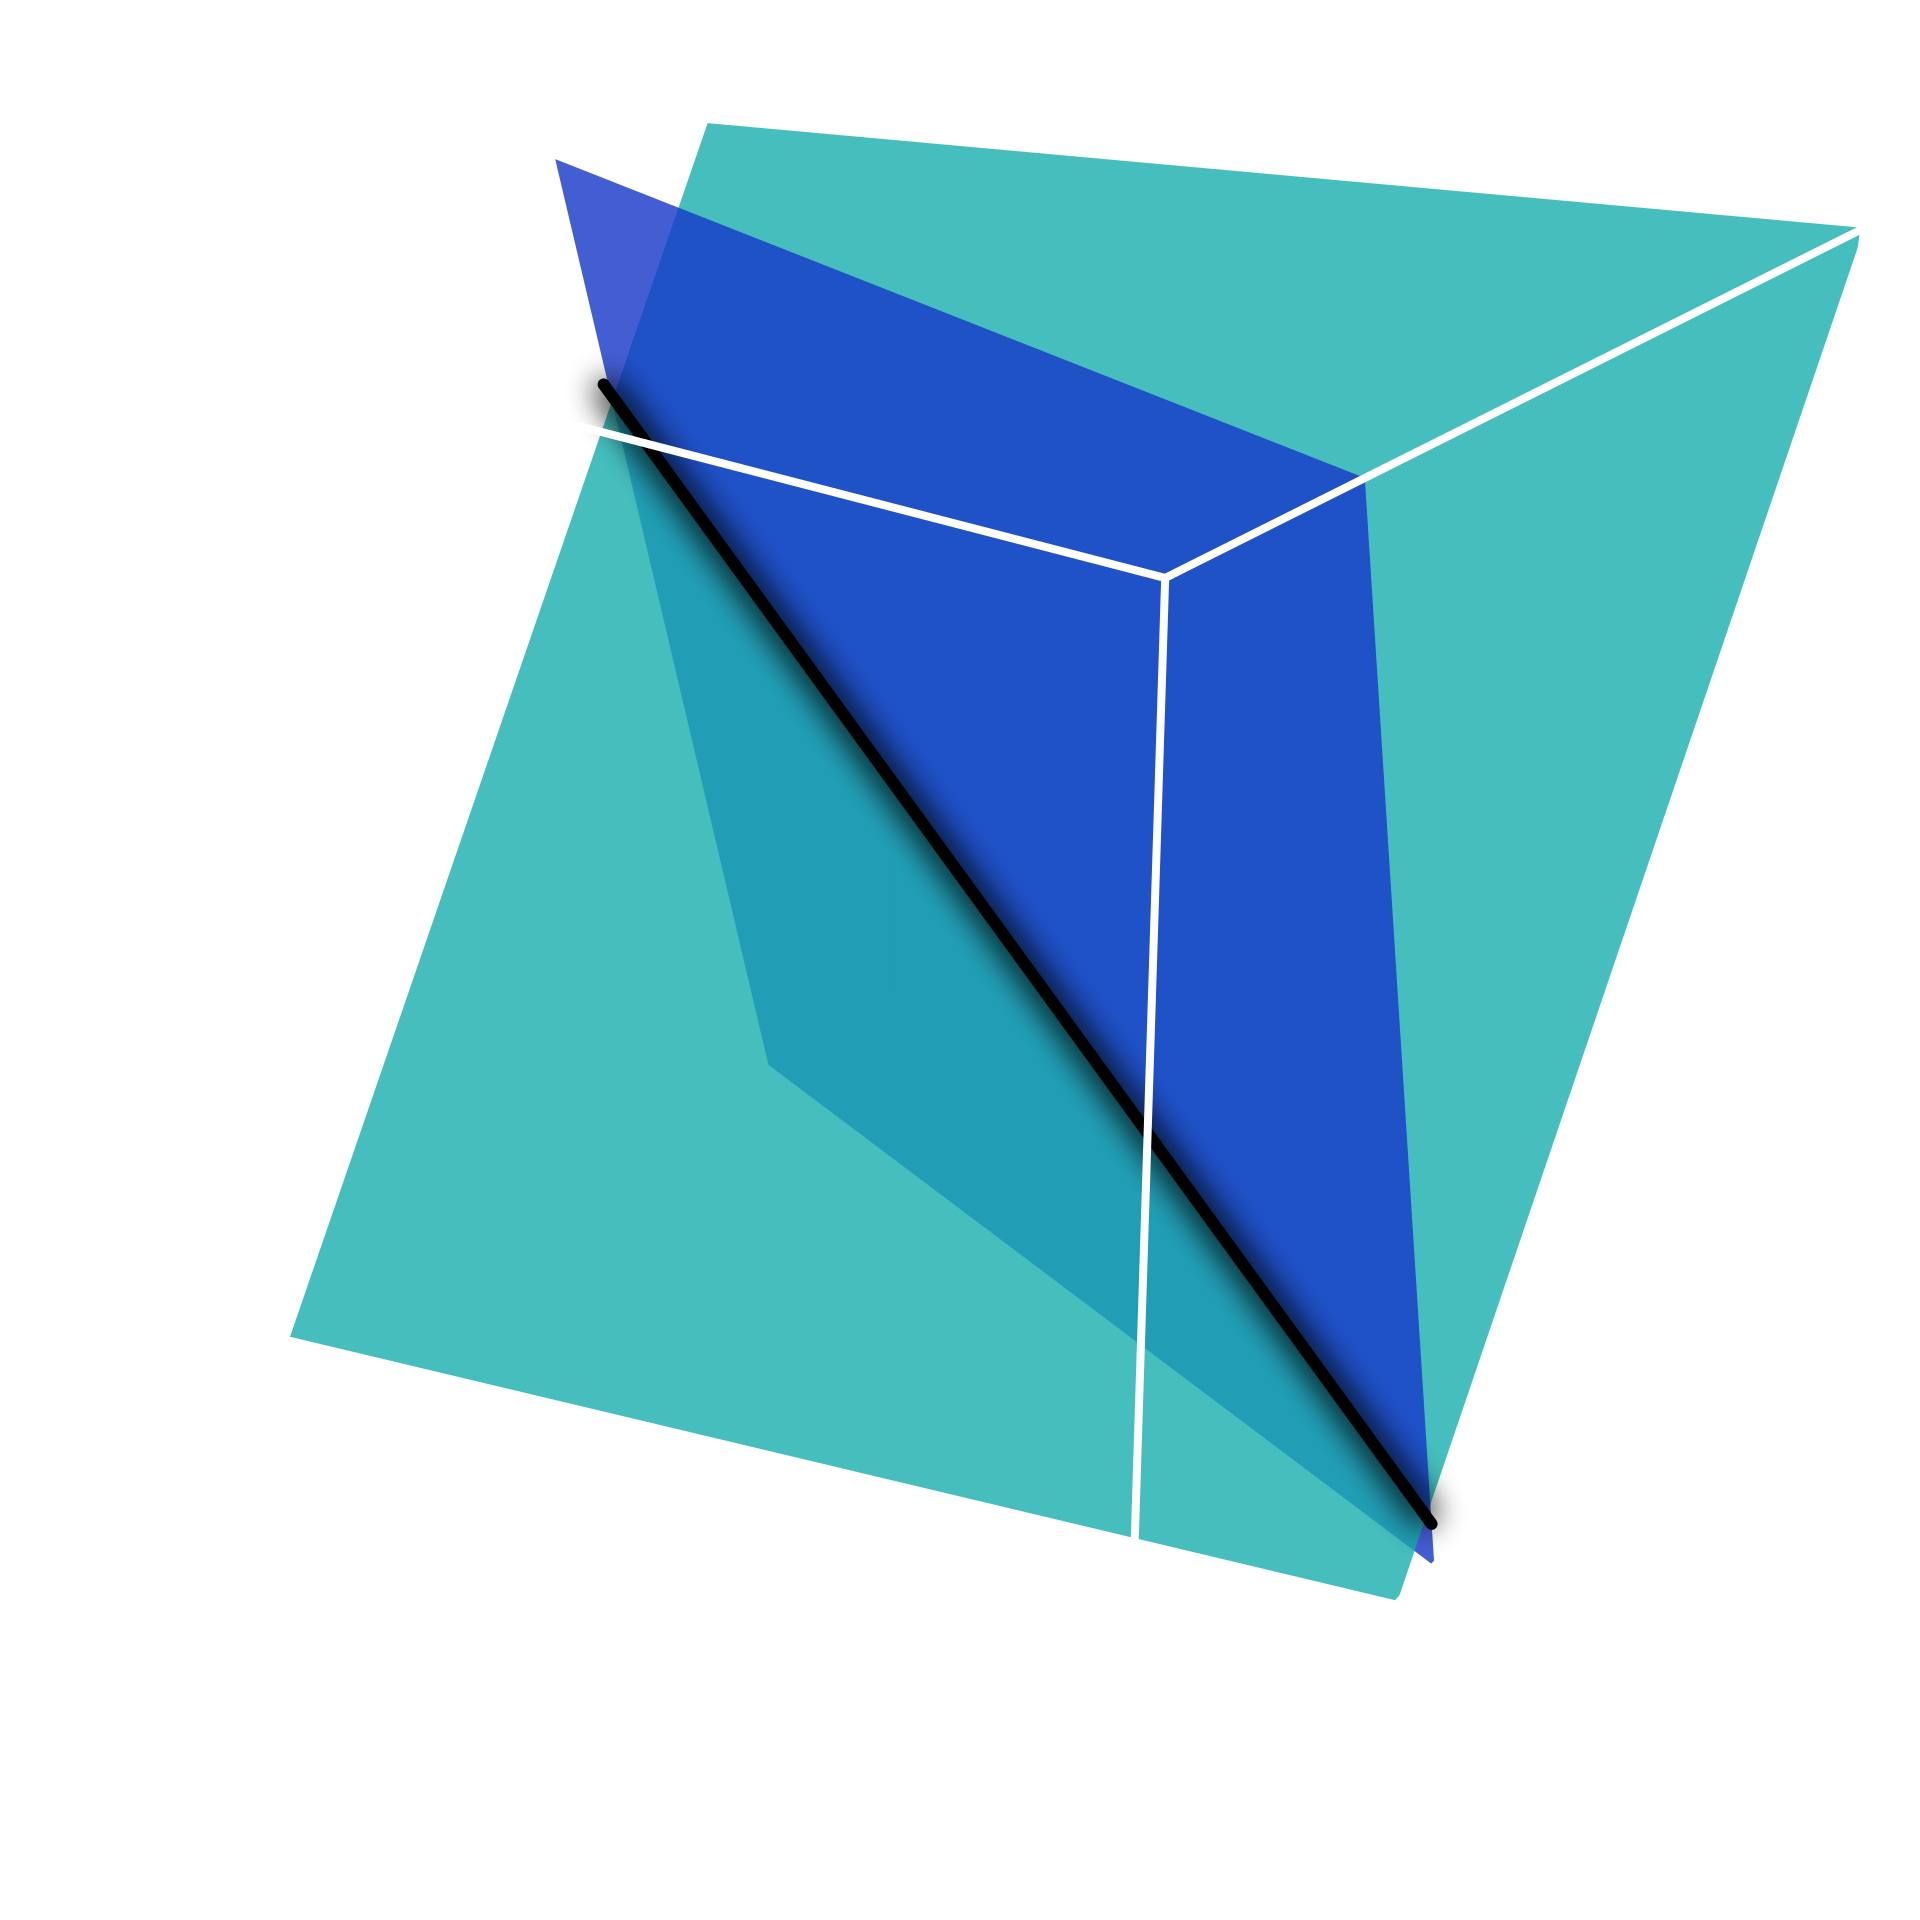
\includegraphics[scale=0.07]{./figures/Intersecting_Planes_2.png}}
	\put(1.945,0){\circle*{0.06}}
	\put(2,0){\small $O$}
	\put(1.6,0.56){\small $\Sigma_1$}
	\put(1.34,-0.4){\small $\Sigma_2$}
	\put(2.2,-0.4){\small $L$}
    \end{picture}
\end{frame}
%-------------- end slide -------------------------------%}}}
%-------------- start slide -------------------------------%{{{ 7
\frame{
\begin{example}
    In $\RR^3$, the line $L$ through the origin that is
    parallel to the vector
    ${\vec d}= \left[ \begin{array}{r} -5 \\ 1 \\ -4 \end{array}\right]$
    has (vector) equation
    $\left[ \begin{array}{r} x \\ y \\ z \end{array}\right]
    =t\left[ \begin{array}{r} -5 \\ 1 \\ -4 \end{array}\right], t\in\RR$,
    so
    \[ L=\left\{ t{\vec d} ~|~ t\in\RR\right\}.\]
    {\bf \textcolor{lgtblue}{Claim.}} $L$ is a subspace of $\RR^3$.
    \begin{itemize}
	\item First: $\vec{0}_3\in L$ since $0{\vec d}=\vec{0}_3$.
	\item Suppose $\vec{u},\vec{v}\in L$.  Then by definition,
	    $\vec{u}=s\vec{d}$ and $\vec{v}=t\vec{d}$, for some
	    $s,t\in\RR$.  Thus
	    \[ \vec{u}+\vec{v} = s\vec{d}+t\vec{d} = (s+t)\vec{d}.\]
	    Since $s+t\in\RR$, $\vec{u}+\vec{v}\in L$; i.e., $L$ is closed under addition.
    \end{itemize}
\end{example}
}
%-------------- end slide -------------------------------%}}}
%-------------- start slide -------------------------------%{{{ 8
\frame{
\begin{example}[continued]
\begin{itemize}
    \item Suppose ${\vec u}\in L$ and $k\in\RR$ ($k$ is a scalar).
	Then $\vec{u}=t\vec{d}$, for some $t\in\RR$, so
	\[ k\vec{u}=k(t\vec{d})=(kt)\vec{d}.\]
	Since $kt\in\RR$, $k\vec{u}\in L$;
	i.e., $L$ is closed under scalar multiplication.
    \item Therefore, $L$ is a subspace of $\RR^3$.
\end{itemize}
\end{example}
\vfill
\pause
\begin{remark}
    Note that there is nothing special about the vector $\vec{d}$ used
    in this example; the same proof works for any \alert{nonzero}
    vector $\vec{d}\in\RR^3$, so any line through the origin is
    a subspace of $\RR^3$.
\end{remark}
}
%-------------- end slide -------------------------------%}}}
%-------------- start slide -------------------------------%{{{ 9
\frame{
\begin{example}
    In $\RR^3$, let $M$ denote the plane through the origin having
    equation $3x-2y+z=0$; then $M$ has normal vector
    ${\vec n}=\left[\begin{array}{r} 3 \\ -2 \\ 1 \end{array}\right]$.
    If ${\vec u}=\left[\begin{array}{r} x \\ y \\ z \end{array}\right]$,
    then
    \[ M= \left\{ {\vec u}\in\RR^3 ~|~ \vec{n}\cdot\vec{u}=0\right\},\]
    where $\vec{n}\cdot\vec{u}$ is the dot product of vectors $\vec n$ and
    $\vec u$.
    \medskip

    {\bf \textcolor{lgtblue}{Claim.}} $M$ is a subspace of $\RR^3$.

    \begin{itemize}
	\item First: $\vec{0}_3\in M$ since $\vec{n}\cdot\vec{0}_3=0$.
	\item Suppose $\vec{u},\vec{v}\in M$.  Then by definition,
	    $\vec{n}\cdot\vec{u}=0$ and $\vec{n}\cdot\vec{v}=0$, so
	    \[ \vec{n}\cdot(\vec{u}+\vec{v}) = n\cdot\vec{u} + n\cdot\vec{v} = 0 + 0 =0, \]
	    and thus $(\vec{u}+\vec{v})\in M$; i.e., $M$ is closed under addition.
    \end{itemize}

\end{example}
}
%-------------- end slide -------------------------------%}}}
%-------------- start slide -------------------------------%{{{ 10
\frame{
    \begin{example}[continued]
\begin{itemize}
    \item Suppose ${\vec u}\in M$ and $k\in\RR$.
	Then $\vec{n}\cdot \vec{u}=0$, so
	\[ {\vec n}\cdot(k{\vec u}) = k(\vec{n}\cdot\vec{u}) = k(0)=0,\]
	and thus $k{\vec u}\in M$; i.e., $M$ is closed under scalar
	multiplication.\\[0.5em]
    \item Therefore, $M$ is a subspace of $\RR^3$.
\end{itemize}
\end{example}
\vfill
\pause
\begin{remark}
    As in the previous example, there is nothing special about the plane
    chosen for this example; any plane through the origin is a subspace
    of $\RR^3$.
\end{remark}
}
%-------------- end slide -------------------------------%}}}
%-------------- start slide -------------------------------%{{{ 11
\frame{
\begin{problem}
    Is
    $U=\left\{\left. \left[\begin{array}{r} a \\ b\\ c\\ d \end{array}
    \right] ~\right|~  a,b,c,d\in\RR\quad\text{and}\quad 2a-b=c+2d \right\}$
    a subspace of $\RR^4$?
    Justify your answer.
\end{problem}
\pause
\vfill
\begin{solution}
    The zero vector of $\RR^4$ is the vector
    $\left[\begin{array}{c} a \\ b \\ c \\ d \end{array}\right]$
    with $a=b=c=d=0$.

    In this case, $2a-b=2(0)+0=0$ and $c+2d=0+2(0)=0$, so $2a-b=c+2d$.
    Therefore, $\vec{0}_4\in U$.
    \myQED
\end{solution}
}
%-------------- end slide -------------------------------%}}}
%-------------- start slide -------------------------------%{{{ 12
\frame{
\begin{solution}[continued]
    Suppose
    \[ \vec{v}_1=\left[\begin{array}{c} a_1 \\ b_1 \\ c_1 \\ d_1 \end{array}\right]
    \quad\text{and}\quad
    \vec{v}_2=\left[\begin{array}{c} a_2 \\ b_2 \\ c_2 \\ d_2 \end{array}\right]
    \mbox{ are in } U.\]
    Then $2a_1-b_1=c_1+2d_1$ and $2a_2-b_2=c_2+2d_2$.
    Now
    \[
	\vec{v}_1+\vec{v}_2 = \left[\begin{array}{c} a_1 \\ b_1 \\ c_1 \\ d_1 \end{array}\right] +
    \left[\begin{array}{c} a_2 \\ b_2 \\ c_2 \\ d_2 \end{array}\right]
    =
    \left[\begin{array}{c} a_1+a_2 \\ b_1+b_2 \\ c_1+c_2 \\ d_1+d_2 \end{array}\right],\]
    and
    \begin{eqnarray*}
	2(a_1+a_2) - (b_1+b_2) & = & (2a_1-b_1)+(2a_2-b_2) \\
                               & = & (c_1+2d_1)+(c_2+2d_2) \\
                               & = & (c_1+c_2)+2(d_1+d_2).
    \end{eqnarray*}
    Therefore, $\vec{v}_1+\vec{v}_2\in U$.
\end{solution}
}
%-------------- end slide -------------------------------%}}}
%-------------- start slide -------------------------------%{{{ 13
\frame{
    \begin{solution}[continued]
    Finally, suppose
    \[ \vec{v}=\left[\begin{array}{c} a \\ b \\ c \\ d \end{array}\right] \in U
    \quad\text{and}\quad k\in\RR.\]
    Then $2a-b=c+2d$.
    Now
    \[  k\vec{v} = k\left[\begin{array}{c} a \\ b \\ c \\ d \end{array}\right]
                  = \left[\begin{array}{c} ka \\ kb \\ kc \\ kd \end{array}\right],\]
    and
    \[ 2ka-kb=k(2a-b)=k(c+2d)=kc+2kd.\]
    Therefore, $k\vec{v}\in U$.
    \medskip

    It follows from the \textcolor{yellow}{Subspace Test} that $U$ is a subspace of $\RR^4$.
    \end{solution}
}
%-------------- end slide -------------------------------%}}}
%-------------- start slide -------------------------------%{{{ 14
\frame{
\begin{problem}
    Is $U=\left\{\left. \left[\begin{array}{r} 1 \\ s\\ t \end{array}
    \right] ~\right|~  s,t\in\RR\right\}$
    a subspace of $\RR^3$?  Justify your answer.
\end{problem}
\pause
\vfill
\begin{solution}
    Note that $\vec{0}_3\not \in U$, and thus $U$ is not a subspace of
    $\RR^3$.
    \bigskip

    (You could also show that $U$ is not closed under addition, or
    not closed under scalar multiplication.)
\end{solution}
}
%-------------- end slide -------------------------------%}}}
%-------------- start slide -------------------------------%{{{ 15
\frame{
\begin{problem}
    Is
    $U=\left\{\left. \left[\begin{array}{r} r \\ 0\\ s \end{array}
    \right] ~\right|~  r,s\in\RR\quad\text{and}\quad r^2 + s^2 = 0\right\}$
    a subspace of $\RR^3$?

    Justify your answer.
\end{problem}
\pause
\vfill
\begin{solution}
    Since $r\in\RR$, $r^2\geq 0$ with equality if and only if $r=0$.
    Similarly, $s\in\RR$ implies $s^2\geq 0$, and
    $s^2=0$ if and only if $s=0$.
    This means $r^2+s^2=0$ if and only if $r^2=s^2=0$;
    thus $r^2+s^2=0$ if and only if $r=s=0$.
    Therefore $U$ contains only $\vec{0}_3$, the zero vector,
    i.e., $U=\{\vec{0}_3\}$.
    As we already observed, $\{\vec{0}_n\}$ is a subspace of $\RR^n$,
    and therefore $U$ is a subspace of $\RR^3$.
    \myQED
\end{solution}
}
%-------------- end slide -------------------------------%}}}
\section[\textcolor{yellow}{}]{\textcolor{yellow}{The null space and the image space}}
%-------------- start slide -------------------------------%{{{ 16
\frame{
\frametitle{The null space and the image space}
\pause
\begin{definitions}[Null Space and Image Space]
    Let $A$ be an $m\times n$ matrix.
    The \textcolor{red}{null space} of $A$ is defined as
    \[ \nul(A) = \{ \vec{x}\in\RR^n ~|~ A\vec{x}=\vec{0}_m\},\]
    and the \textcolor{red}{image space} of $A$ is defined as
    \[ \im(A) = \{ A\vec{x}~|~ \vec{x}\in\RR^n \}.\]
\end{definitions}
\vfill
\pause
\begin{remark}
    \begin{enumerate}
        \item Since $A$ is $m\times n$ and $\vec{x}\in\RR^n$,
	    $A\vec{x}\in\RR^m$, so $\im(A) \subseteq \RR^m$ while
	    $\nul(A)\subseteq \RR^n$.
	\item Image space is also called \alert{column space} of $A$, denoted
	    as $\col(A)$:
	    \begin{align*}
		\col(A) = \text{span}\left(\vec{a}_1,\cdots,\vec{a}_n \right) = \im(A).
	    \end{align*}
    \end{enumerate}
\end{remark}
}
%-------------- end slide -------------------------------%}}}
%-------------- start slide -------------------------------%{{{ 17
\frame{
\begin{problem}
    Prove that if $A$ is an $m\times n$ matrix, then $\nul(A)$ is a subspace of $\RR^n$.
\end{problem}
\pause
\begin{proofnoend}
\begin{itemize}
    \item[S1.] Since $A\vec{0}_n=\vec{0}_m$, $\vec{0}_n\in\nul(A)$.
    \pause
    \item[S2.] Let $\vec{x},\vec{y}\in\nul(A)$.  Then $A\vec{x}=\vec{0}_m$ and $A\vec{y}=\vec{0}_m$, so
    \[ A(\vec{x}+\vec{y})=A\vec{x}+A\vec{y} = \vec{0}_m+\vec{0}_m=\vec{0}_m,\]
    and thus $\vec{x}+\vec{y}\in\nul(A)$.
    \pause
    \item[S3.] Let $\vec{x}\in\nul(A)$ and $k\in\RR$. Then $A\vec{x}=\vec{0}_m$, so
    \[ A(k\vec{x}) = k(A\vec{x})=k\vec{0}_m=\vec{0}_m,\]
    and thus $k\vec{x}\in\nul(A)$.
\end{itemize}
Therefore, $\nul(A)$ is a subspace of $\RR^n$.
\myQED\end{proofnoend}
}
%-------------- end slide -------------------------------%}}}
%-------------- start slide -------------------------------%{{{ 18
\frame{
\begin{problem}
    Prove that if $A$ is an $m\times n$ matrix, then $\im(A)$ is a subspace of $\RR^m$.
\end{problem}
\pause
\begin{proofnoend}
\begin{itemize}
    \item[S1.] Since $\vec{0}_n\in\RR^n$ and $A\vec{0}_n=\vec{0}_m$, $\vec{0}_m\in\im(A)$.
    \pause
    \item[S2.] Let $\vec{x},\vec{y}\in\im(A)$.  Then $\vec{x}=A\vec{u}$ and $\vec{y}=A\vec{v}$ for some $\vec{u},\vec{v}\in\RR^n$, so
    \[ \vec{x}+\vec{y}=A\vec{u}+A\vec{v} = A(\vec{u}+\vec{v}).\]
    Since $\vec{u}+\vec{v}\in\RR^n$, it follows that $\vec{x}+\vec{y}\in\im(A)$.
    \pause
    \item[S3.] Let $\vec{x}\in\im(A)$ and $k\in\RR$.
    Then $\vec{x}=A\vec{u}$ for some $\vec{u}\in\RR^n$, and thus
    \[ k\vec{x} = k(A\vec{u}) = A(k\vec{u}).\]
    Since $k\vec{u}\in\RR^n$, it follows that $k\vec{x}\in\im(A)$.
\end{itemize}
Therefore, $\im(A)$ is a subspace of $\RR^m$.
\myQED\end{proofnoend}
}
%-------------- end slide -------------------------------%}}}
\section[\textcolor{yellow}{}]{\textcolor{yellow}{The Eigenspace}}
%-------------- start slide -------------------------------%{{{ 19
\frame{
\frametitle{The Eigenspace}
\pause
\begin{definition}[Eigenspace]
    Let $A$ be an $n\times n$ matrix and $\lambda\in\RR$.
    The \textcolor{red}{eigenspace of $A$ corresponding to $\lambda$}
    is the set
    \[ E_{\lambda}(A) = \left\{ \vec{x}\in\RR^n ~|~ A\vec{x}=\lambda\vec{x} \right\}. \]
\end{definition}
}
%-------------- end slide -------------------------------%}}}
%-------------- start slide -------------------------------%{{{ 20
\begin{frame}[fragile]
    \begin{example}
	$A=\begin{pmatrix} 4&-2\cr -1&3 \end{pmatrix} $ has two eigenvalues:
	$\lambda_1=2$ and $\lambda_2=5$ with corresponding eigenvectors
	\begin{align*}
	    \vec{v}_1 =\begin{pmatrix} 1\cr 1 \end{pmatrix}
	    \quad\text{and}\quad
	    \vec{v}_2 =\begin{pmatrix} -1\cr 1/2 \end{pmatrix}
	\end{align*}
	\bigskip
	Hence,
	\begin{align*}
	    E_{\lambda_1}(A) = E_{2}(A) = \left\{ t \vec{v}_1| t\in\R \right\} \\
	    E_{\lambda_2}(A) = E_{5}(A) = \left\{ t \vec{v}_2| t\in\R \right\} \\
	\end{align*}
    \end{example}

\end{frame}
%-------------- end slide -------------------------------%}}}
%-------------- start slide -------------------------------%{{{ 21
\begin{frame}[fragile]
\begin{center}
    \begin{center}
        \begin{tikzpicture}[scale=0.7, transform shape]
        \tikzset{>=latex}
	\draw [->] (-5.5,0) -- (6.5,0) node [right] {$x$};
	\draw [->] (0,-4.5) -- (0,6.5) node [above] {$y$};
	\foreach \x in {-5,...,-1} {
	    \draw (\x,0.1) -- (\x,-0.1) node [below] {$\x$};
	}
	\foreach \x in {1,...,6} {
	    \draw (\x,0.1) -- (\x,-0.1) node [below] {$\x$};
	}
	\foreach \y in {-4,...,-1} {
	    \draw (0.1,\y) -- (-0.1,\y) node [left] {$\y$};
	}
	\foreach \y in {1,...,6} {
	    \draw (0.1,\y) -- (-0.1,\y) node [left] {$\y$};
	}

	\foreach \x in {-5,...,6}{
	    \draw [dotted,gray] (\x,-4.5) -- (\x,6.5);
	}
	\foreach \y in {-4,...,6}{
	    \draw [dotted,gray] (-5.5,\y) -- (6.5,\y);
	}
	\node at (3,7) {$A=\begin{pmatrix} 4&-2\cr -1&3 \end{pmatrix} $};
	\coordinate (A) at (4,-1);
	\coordinate (O) at (0,0);
	\coordinate (B) at (-2,3);
	\pause
	\draw [blue,->,thick] (O) -- (1,0);
	\pause
	\draw [red,->,thick] (O) -- (A);
	\pause
	\draw [blue,->,thick] (O) -- (0,1);
	\pause
	\draw [red,->,thick] (O) -- (B);
	\pause
	\begin{scope}
	    \clip(-5.5,-4.5) rectangle (6.5,6.5);
	    \foreach \i in {-2,0,2,4} {
		\draw [shorten >= -10cm,shorten <= -10cm,dashed,gray] (\i,\i)  -- +($(A)-(O)$);
		\draw [shorten >= -10cm,shorten <= -10cm,dashed,gray] (\i,\i)  -- +($(B)-(O)$);
		}
	    % \draw [shorten >= -10cm,shorten <= -10cm,dashed] (0,5)  -- +($(A)-(O)$);
	    % \draw [shorten >= -10cm,shorten <= -10cm,dashed] (0,5)  -- +($(B)-(O)$);
	\end{scope}
	\pause
	\draw [yellow,->] (0,0) -- (2,1);
	\pause
	\draw [magenta,->] (0,0) -- (6,1);
	\pause
	\draw [yellow,->] (0,0) -- (1,-1);
	\pause
	\draw [magenta,->] (0,0) -- (6,-4);
	\pause
	\draw [yellow,->] (0,0) -- (1,1);
	\pause
	\draw [magenta,->] (0,0) -- (2,2);
	\pause
	\begin{scope}
	    \clip(-5.5,-4.5) rectangle (6.5,6.5);
	    \draw [shorten >= -10cm,shorten <= -10cm,lgtblue,very thick] (0,0) -- (1,1);
	\end{scope}
	\node [lgtblue] at (7,6.8) {$E_{\lambda_1}(A)$};
	\pause
	\draw [yellow,->] (0,0) -- (-1,0.5);
	\pause
	\draw [magenta,->] (0,0) -- (-5,2.5);
	\pause
	\begin{scope}
	    \clip(-5.5,-4.5) rectangle (6.5,6.5);
	    \draw [shorten >= -10cm,shorten <= -10cm,lgtblue,very thick] (0,0) --(-2,1);
	\end{scope}
	\node [lgtblue] at (7,-3.5) {$E_{\lambda_2}(A)$};
        \end{tikzpicture}
    \end{center}
\end{center}
\end{frame}
%-------------- end slide -------------------------------%}}}
%-------------- start slide -------------------------------%{{{ 22
\begin{frame}[fragile]
\begin{center}
    \begin{center}
        \begin{tikzpicture}[scale=0.7, transform shape]
        \tikzset{>=latex}
	\draw [->] (-5.5,0) -- (6.5,0) node [right] {$x$};
	\draw [->] (0,-4.5) -- (0,6.5) node [above] {$y$};
	\foreach \x in {-5,...,-1} {
	    \draw (\x,0.1) -- (\x,-0.1) node [below] {$\x$};
	}
	\foreach \x in {1,...,6} {
	    \draw (\x,0.1) -- (\x,-0.1) node [below] {$\x$};
	}
	\foreach \y in {-4,...,-1} {
	    \draw (0.1,\y) -- (-0.1,\y) node [left] {$\y$};
	}
	\foreach \y in {1,...,6} {
	    \draw (0.1,\y) -- (-0.1,\y) node [left] {$\y$};
	}

	\foreach \x in {-5,...,6}{
	    \draw [dotted,gray] (\x,-4.5) -- (\x,6.5);
	}
	\foreach \y in {-4,...,6}{
	    \draw [dotted,gray] (-5.5,\y) -- (6.5,\y);
	}
	\node at (3,7) {$A=\begin{pmatrix} 4&-2\cr -1&3 \end{pmatrix} $};
	\coordinate (A) at (4,-1);
	\coordinate (O) at (0,0);
	\coordinate (B) at (-2,3);
	% \pause
	% \draw [blue,->,thick] (O) -- (1,0);
	% \pause
	% \draw [red,->,thick] (O) -- (A);
	% \pause
	% \draw [blue,->,thick] (O) -- (0,1);
	% \pause
	% \draw [red,->,thick] (O) -- (B);
	% \pause
	\begin{scope}
	    \clip(-5.5,-4.5) rectangle (6.5,6.5);
	    \foreach \i in {-2,0,2,4} {
		\draw [shorten >= -10cm,shorten <= -10cm,dashed,gray] (\i,\i)  -- +($(A)-(O)$);
		\draw [shorten >= -10cm,shorten <= -10cm,dashed,gray] (\i,\i)  -- +($(B)-(O)$);
		}
	    % \draw [shorten >= -10cm,shorten <= -10cm,dashed] (0,5)  -- +($(A)-(O)$);
	    % \draw [shorten >= -10cm,shorten <= -10cm,dashed] (0,5)  -- +($(B)-(O)$);
	\end{scope}
	% \pause
	% \draw [yellow,->] (0,0) -- (2,1);
	% \pause
	% \draw [magenta,->] (0,0) -- (6,1);
	% \pause
	% \draw [yellow,->] (0,0) -- (1,-1);
	% \pause
	% \draw [magenta,->] (0,0) -- (6,-4);
	% \pause
	% \draw [yellow,->] (0,0) -- (1,1);
	% \pause
	% \draw [magenta,->] (0,0) -- (2,2);
	% \pause
	\begin{scope}
	    \clip(-5.5,-4.5) rectangle (6.5,6.5);
	    \draw [shorten >= -10cm,shorten <= -10cm,lgtblue,very thick] (0,0) -- (1,1);
	\end{scope}
	\node [lgtblue] at (9,6.5) {$E_{2}(A) =  \left\{t \begin{pmatrix} 1\\ 1 \end{pmatrix} \bigg| t\in\R \right\}$};
	% \pause
	% \draw [yellow,->] (0,0) -- (-1,0.5);
	% \pause
	% \draw [magenta,->] (0,0) -- (-5,2.5);
	% \pause
	\begin{scope}
	    \clip(-5.5,-4.5) rectangle (6.5,6.5);
	    \draw [shorten >= -10cm,shorten <= -10cm,lgtblue,very thick] (0,0) --(-2,1);
	\end{scope}
	\node [lgtblue] at (9,-3.3) {$E_{5}(A) = \left\{t \begin{pmatrix} -1\\ 1/2 \end{pmatrix} \bigg| t\in\R \right\}$};
        \end{tikzpicture}
    \end{center}
\end{center}
\end{frame}
%-------------- end slide -------------------------------%}}}
%-------------- start slide -------------------------------%{{{ 23
\begin{frame}[fragile]
\begin{emptytitle}
    Note that
    \begin{eqnarray*}
	E_{\lambda}(A)
	& = & \left\{ \vec{x}\in\RR^n ~|~ A\vec{x}=\lambda\vec{x} \right\}               \\
	& = & \left\{ \vec{x}\in\RR^n ~|~ \lambda\vec{x}  - A\vec{x}=\vec{0}_n \right\} \\
	& = & \left\{ \vec{x}\in\RR^n ~|~ (\lambda I - A)\vec{x}=\vec{0}_n \right\}
    \end{eqnarray*}
    showing that
    \[  E_{\lambda}(A) = \nul(\lambda I-A).\]
    \pause
    It follows that
    \begin{itemize}
    \item if $\lambda$ is \textcolor{red}{not} an eigenvalue of $A$,
    then $E_{\lambda}(A)=\{\vec{0}_n\}$;
    \item the nonzero vectors of $E_{\lambda}(A)$ are the
    eigenvectors of $A$ corresponding to $\lambda$;
    \item
    the eigenspace of $A$ corresponding to $\lambda$
    is a subspace of $\RR^n$.
    \end{itemize}
\end{emptytitle}
\end{frame}
%-------------- end slide -------------------------------%}}}
\section[\textcolor{yellow}{}]{\textcolor{yellow}{Linear Combinations and Spanning Sets}}
%-------------- start slide -------------------------------%{{{ 24
\frame{
\frametitle{Linear Combinations and Spanning Sets}
\pause
\begin{definition}[Linear Combinations and Spanning]
    Let $\vec{x}_1, \vec{x}_2, \ldots, \vec{x}_k\in\RR^n$ and $t_1, t_2, \ldots, t_k\in\RR$.
    Then the vector
    \[ \vec{x} = t_1\vec{x}_1 + t_2\vec{x}_2 + \cdots + t_k\vec{x}_k \]
    is called a \textcolor{red}{linear combination} of the vectors $\vec{x}_1, \vec{x}_2, \ldots, \vec{x}_k$;
    the (scalars) $t_1, t_2, \ldots, t_k\in\RR$ are the {\bf coefficients}.
    The set of {\bf all} linear combinations of
    $\vec{x}_1, \vec{x}_2, \ldots, \vec{x}_k$ is called
    \textcolor{red}{the span of $\vec{x}_1, \vec{x}_2, \ldots, \vec{x}_k$}, and is written
    \[
	\Span \{\vec{x}_1, \vec{x}_2, \ldots, \vec{x}_k\}
	= \left\{ t_1\vec{x}_1 + t_2\vec{x}_2 + \cdots + t_k\vec{x}_k ~|~ t_1, t_2, \ldots, t_k\in\RR\right\}.
    \]
\end{definition}
\pause
\vfill

\begin{emptytitle}{\bf Additional Terminology.}
    If $U=\Span \{\vec{x}_1, \vec{x}_2, \ldots, \vec{x}_k\}$, then
    \begin{itemize}
	\item \textcolor{red}{$U$ is spanned by} the vectors $\vec{x}_1, \vec{x}_2, \ldots, \vec{x}_k$.
	\item the vectors $\vec{x}_1, \vec{x}_2, \ldots, \vec{x}_k$ \textcolor{red}{span $U$}.
	\item the set of vectors $\{ \vec{x}_1, \vec{x}_2, \ldots, \vec{x}_k\}$ is a \textcolor{red}{spanning set} for $U$.
    \end{itemize}
\end{emptytitle}
}
%-------------- end slide -------------------------------%}}}
%-------------- start slide -------------------------------%{{{ 25
\frame{
\begin{example}
    Let $\vec{x}\in\RR^3$ be a nonzero vector.
    Then $\Span\{\vec{x}\} = \{ k\vec{x} ~|~ k\in\RR\}$
    is a line through the origin having direction vector $\vec{x}$.
\end{example}
\pause

\begin{example}
    Let $\vec{x},\vec{y}\in\RR^3$ be nonzero vectors that are not
    parallel.
    Then
    \[ \Span\{\vec{x},\vec{y}\} = \{ k\vec{x} + t\vec{y} ~|~ k,t\in\RR\} \]
    is a plane through the origin containing $\vec{x}$ and $\vec{y}$.
    \pause
    \medskip

    \textcolor{blue}{How would you find the equation of this plane?}
\end{example}
}
%-------------- end slide -------------------------------%}}}
%-------------- start slide -------------------------------%{{{ 26
\frame{
\begin{problem}
    Let
    $\vec{x}=\left[ \begin{array}{r} 8 \\ 3 \\ -13 \\ 20 \end{array}\right]$,
    $\vec{y}=\left[ \begin{array}{r} 2 \\ 1 \\ -3 \\ 5 \end{array}\right]$
    and
    $\vec{z}=\left[ \begin{array}{r} -1 \\ 0 \\ 2 \\ -3 \end{array}\right]$.
    Is $\vec{x}\in\Span\{\vec{y},\vec{z}\}$?
\end{problem}
\pause
\begin{solution}
    An equivalent question is:
    can $\vec{x}$ be expressed as a linear combination of $\vec{y}$ and
    $\vec{z}$?

    Suppose there exist $a,b\in\RR$ so that $\vec{x}=a\vec{y}+b\vec{z}$.
    Then
    \[
    \left[ \begin{array}{r} 8 \\ 3 \\ -13 \\ 20 \end{array}\right]
    = a \left[ \begin{array}{r} 2 \\ 1 \\ -3 \\ 5 \end{array}\right] + b\left[ \begin{array}{r} -1 \\ 0 \\ 2 \\ -3 \end{array}\right]
    = \left[ \begin{array}{rr} 2 & -1 \\ 1 & 0 \\ -3 & 2 \\ 5 & -3 \end{array}\right]
    \left[ \begin{array}{c} a \\ b \end{array}\right].
    \]
    Solve this system of four linear equations in the two variables
    $a$ and $b$.
\end{solution}
}
%-------------- end slide -------------------------------%}}}
%-------------- start slide -------------------------------%{{{ 27
\frame{
\begin{solution}[continued]
    \[
    \left[ \begin{array}{rr|r}
    2 & -1 & 8 \\ 1 & 0 & 3 \\ -3 & 2 & -13 \\ 5 & -3 & 20 \end{array}\right]
    \rightarrow
    \left[ \begin{array}{rr|r}
    1 & 0 & 3 \\ 0 & 1 & -2 \\ 0 & 0 & 0 \\ 0 & 0 & -1 \end{array}\right]
    \]
    Since the system has no solutions, $\vec{x}\not\in\Span\{\vec{y},\vec{z}\}$.
    \myQED
\end{solution}
}
%-------------- end slide -------------------------------%}}}
%-------------- start slide -------------------------------%{{{ 28
\frame{
\begin{problem}
    Let
    $\vec{w}=\left[ \begin{array}{r} 8 \\ 3 \\ -13 \\
    \alert{21} \end{array}\right]$,
    $\vec{y}=\left[ \begin{array}{r} 2 \\ 1 \\ -3 \\ 5 \end{array}\right]$
    and
    $\vec{z}=\left[ \begin{array}{r} -1 \\ 0 \\ 2 \\ -3 \end{array}\right]$.
    Is $\vec{w}\in\Span\{\vec{y},\vec{z}\}$?
    \medskip

    \alert{This is almost identical to a previous problem, except that
    $\vec{w}$ (above) has one entry that is different from the
    vector $\vec{x}$ of that problem.}
\end{problem}
\pause
\vfill
\begin{solution}
    In this case, the system of linear equations is consistent, and
    gives us $\vec{w}=3\vec{y}-2\vec{z}$, so $\vec{w}\in\Span\{\vec{y},\vec{z}\}$.
\end{solution}
}
%-------------- end slide -------------------------------%}}}
%-------------- start slide -------------------------------%{{{ 29
\frame{
\begin{theorem}
    Let $\vec{x}_1, \vec{x}_2, \ldots, \vec{x}_k\in\RR^n$ and let
    $U=\Span \{ \vec{x}_1, \vec{x}_2, \ldots, \vec{x}_k \}$. Then
    \begin{enumerate}
	\item $U$ is a subspace of $\RR^n$ containing each $\vec{x}_i$, $1\leq i\leq k$;
	\item if $W$ is a subspace of $\RR^n$ and $\vec{x}_1, \vec{x}_2, \ldots, \vec{x}_k\in W$, then $U\subseteq W$.
    \end{enumerate}
\end{theorem}
\pause
\vfill
\begin{remark}
    Property 2 is saying that $U$ is the ``smallest'' subspace
    of $\RR^n$ that contains $\vec{x}_1, \vec{x}_2, \ldots, \vec{x}_k$.
\end{remark}

}
%-------------- end slide -------------------------------%}}}
%-------------- start slide -------------------------------%{{{ 30
\begin{frame}[fragile]

\begin{proofnoend}[ Part 1 of Theorem ]
    Since $U=\Span \{ \vec{x}_1, \vec{x}_2, \ldots, \vec{x}_k\}$ and
    $0\vec{x}_1 + 0\vec{x}_2 + \cdots + 0\vec{x}_k=\vec{0}_n$,
    \textcolor{yellow}{$\vec{0}_n\in U$.}
    \pause
    \bigskip

    Suppose $\vec{x},\vec{y}\in U$.
    Then for some $s_i,t_i\in\RR$, $1\leq i\leq k$,
    \begin{align*}
	\vec{x}&=s_1\vec{x}_1 + s_2\vec{x}_2 + \cdots + s_k\vec{x}_k  \\
	\vec{y}&=t_1\vec{x}_1 + t_2\vec{x}_2 + \cdots + t_k\vec{x}_k
    \end{align*}
    Thus
    \begin{align*}
	\vec{x}+\vec{y} & =  (s_1\vec{x}_1 + s_2\vec{x}_2 + \cdots + s_k\vec{x}_k)
	+(t_1\vec{x}_1 + t_2\vec{x}_2 + \cdots + t_k\vec{x}_k) \\
	& =  (s_1+t_1)\vec{x}_1 + (s_2+t_2)\vec{x}_2 + \cdots + (s_k+t_k)\vec{x}_k.
    \end{align*}

    Since $s_i+t_i\in\RR$ for all $1\leq i\leq k$,
    $\vec{x}+\vec{y}\in U$, i.e., \textcolor{yellow}{$U$ is closed under addition.}
\end{proofnoend}


\end{frame}
%-------------- end slide -------------------------------%}}}
%-------------- start slide -------------------------------%{{{ 31
\frame{
\begin{proofnoend}[ Part 1 of Theorem -- continued]
    Suppose $\vec{x}\in U$ and $a\in\RR$.
    Then for some $s_i\in\RR$, $1\leq i\leq k$,
    \begin{align*}
        \vec{x}=s_1\vec{x}_1 + s_2\vec{x}_2 + \cdots + s_k\vec{x}_k
    \end{align*}
    Thus
    \begin{eqnarray*}
    a\vec{x} & = & a(s_1\vec{x}_1 + s_2\vec{x}_2 + \cdots + s_k\vec{x}_k)\\
     & = & (as_1)\vec{x}_1 + (as_2)\vec{x}_2 + \cdots + (as_k)\vec{x}_k.
    \end{eqnarray*}
    Since $as_i\in\RR$ for all $1\leq i\leq k$,
    $a\vec{x}\in U$. Hence, \textcolor{yellow}{$U$ is closed under scalar multiplication.}
\bigskip
\pause

    Therefore, $U$ is a subspace of $\RR^n$.
    Furthermore, since
    \[ \vec{x}_i=\sum_{j=1}^{i-1} 0\vec{x}_j +
    1\vec{x}_i +\sum_{j=i+1}^{k} 0\vec{x}_j,\]
    it follows that $\vec{x}_i\in U$ for all $i$, $1\leq i\leq k$.
    \pause
    \vfill

\end{proofnoend}
}
%-------------- end slide -------------------------------%}}}
%-------------- start slide -------------------------------%{{{ 32
\begin{frame}[fragile]

    \begin{proofnoend}[Part 2 of Theorem]
	Let $W\subset\RR^n$ be a subspace that contains $\vec{x}_1,\cdots,\vec{x}_n$.
	We need to prove that $U\subseteq W$.

	\bigskip
	\pause
    Suppose $\vec{x}\in U$.
    Then $\vec{x}=s_1\vec{x}_1 + s_2\vec{x}_2 + \cdots + s_k\vec{x}_k$
    for some $s_i\in\RR$, $1\leq i\leq k$.
    Since $W$ contain each $\vec{x}_i$ and $W$ is closed under
    scalar multiplication,
    it follows that $s_i\vec{x}_i\in W$ for each $i$, $1\leq i\leq k$.
    Furthermore, since $W$ is closed under addition,
    $\vec{x}=s_1\vec{x}_1 + s_2\vec{x}_2 + \cdots + s_k\vec{x}_k\in W$.
    Therefore, $U\subseteq W$.
\end{proofnoend}

\end{frame}
%-------------- end slide -------------------------------%}}}
%-------------- start slide -------------------------------%{{{ 33
\frame{
\begin{problem}[revisited]
    Is
    $U=\left\{\left. \left[\begin{array}{r} a \\ b\\ c\\ d \end{array}
    \right] ~\right|~  a,b,c,d\in\RR\quad\text{and}\quad 2a-b=c+2d \right\}$
    a subspace of $\RR^4$?
    Justify your answer.
\end{problem}
\pause

\begin{solution}[Another]
    Let $\vec{v}=\left[\begin{array}{r} a \\ b\\ c\\ d \end{array}
    \right]\in U$.
    Since $2a-b=c+2d$, $c=2a-b-2d$, and thus
    \[ U=\left\{\left. \left[\begin{array}{c} a \\ b\\ 2a-b-2d\\ d \end{array}
	\right] ~\right|~  a,b,d\in\RR\right\}
	=\Span\left\{
	    \left[\begin{array}{r} 1 \\ 0\\ 2\\ 0 \end{array}\right],
	    \left[\begin{array}{r} 0 \\ 1\\ -1\\ 0 \end{array}\right],
	\left[\begin{array}{r} 0 \\ 0\\ -2\\ 1 \end{array}\right] \right\} .\]
	By a previous {\bf Theorem}, $U$ is a subspace of $\RR^4$.
    \end{solution}
}
%-------------- end slide -------------------------------%}}}
%-------------- start slide -------------------------------%{{{ 34
\frame{
\begin{problem}
    Let $\vec{x},\vec{y}\in\RR^n$,
    $U_1= \Span\{\vec{x},\vec{y}\}$, and $U_2 = \Span\{2\vec{x}-\vec{y},
    2\vec{y}+\vec{x}\}$.
    Prove that $U_1=U_2$.
\end{problem}
\pause
\vfill
\begin{solution}
    \alert{To show that $U_1=U_2$,
    prove that
    $U_1\subseteq U_2, \quad\text{and}\quad
    U_2\subseteq U_1$.}
    We begin by noting that, by the first part of the previous {\bf Theorem},
    $U_1$ and $U_2$ are subspaces of $\RR^n$.
    \pause
    \medskip

    Since $2\vec{x}-\vec{y}, 2\vec{y}+\vec{x}\in U_1$,
    it follows \alert{from the second part of the previous {\bf Theorem}}
    that $\Span\{2\vec{x}-\vec{y}, 2\vec{y}+\vec{x}\}\subseteq U_1$, i.e.,
    $U_2\subseteq U_1$.
    \medskip

    Also, since
    \begin{eqnarray*}
    \vec{x} & = & \frac{2}{5}\left( 2\vec{x}-\vec{y}\right) +
    \frac{1}{5}\left(2\vec{y}+\vec{x}\right), \\
    \vec{y} & = & -\frac{1}{5}\left( 2\vec{x}-\vec{y}\right) +
    \frac{2}{5}\left(2\vec{y}+\vec{x}\right),
    \end{eqnarray*}

    $\vec{x},\vec{y}\in U_2$.
    Therefore,
    \alert{by the second part of the previous {\bf Theorem}},
    $\Span\{\vec{x},\vec{y}\}\subseteq U_2$,
    i.e., $U_1\subseteq U_2$.
    The result now follows.
\end{solution}
}
%-------------- end slide -------------------------------%}}}
%-------------- start slide -------------------------------%{{{ 35
\frame{
\begin{problem}
    Show that $\RR^n=\Span\{ \vec{e}_1, \vec{e}_2, \ldots, \vec{e}_n \}$, where
    $\vec{e}_j$ denote the $j^{th}$ column of $I_n$.
\end{problem}
\pause
\vfill
\begin{solution}
    Let $\vec{x}=\left[ \begin{array}{c}
    x_1 \\ x_2 \\ \vdots \\ x_n \end{array}\right]\in \RR^n$.
    Then
    $\vec{x} = x_1\vec{e_1} + x_2\vec{e_2} + \cdots + x_n\vec{e_n}$,
    where $x_1, x_2, \ldots, x_n\in\RR$.
    Therefore,
    $\vec{x}\in \Span\{ \vec{e}_1, \vec{e}_2, \ldots, \vec{e}_n \}$,
    and thus
    $\RR^n\subseteq \Span\{ \vec{e}_1, \vec{e}_2, \ldots, \vec{e}_n \}$.

    \bigskip
    \pause

    Conversely, since $\vec{e}_i\in\RR^n$ for each $i$, $1\leq i\leq n$
    (and $\RR^n$ is a vector space), it follows that
    $\Span\{ \vec{e}_1, \vec{e}_2, \ldots, \vec{e}_n \} \subseteq \RR^n$.
    The equality now follows.
\end{solution}
}
%-------------- end slide -------------------------------%}}}
%-------------- start slide -------------------------------%{{{ 36
\frame{
\begin{problem}
    Let
    $\vec{x}_1 = \left[\begin{array}{r} 1 \\ 1\\ 1\\ 1 \end{array}\right],
    \vec{x}_2  = \left[\begin{array}{r} 0 \\ 1\\ 1\\ 1 \end{array}\right],
    \vec{x}_3  = \left[\begin{array}{r} 0 \\ 0\\ 1\\ 1 \end{array}\right],
    \vec{x}_4  = \left[\begin{array}{r} 0 \\ 0\\ 0\\ 1 \end{array}\right]$.

    Does $\{ \vec{x}_1, \vec{x}_2, \vec{x}_3, \vec{x}_4 \}$ span $\RR^4$?
    (Equivalently, is $\Span \{ \vec{x}_1, \vec{x}_2, \vec{x}_3, \vec{x}_4 \}=\RR^4$?)
\end{problem}
\pause
\vfill
\begin{solution}
    To prove $\Span \{ \vec{x}_1,\vec{x}_2,\vec{x}_3,\vec{x}_4 \} =\R^4$, we need to prove two directions:
    \begin{align*}
	\Span \{ \vec{x}_1,\vec{x}_2,\vec{x}_3,\vec{x}_4 \} \subseteq \RR^4\quad\text{and}\quad
	\RR^4\subseteq \Span \{ \vec{x}_1,\vec{x}_2,\vec{x}_3,\vec{x}_4 \} .
    \end{align*}
    \pause

    For the first relation, since $\vec{x}_1, \vec{x}_2, \vec{x}_3, \vec{x}_4 \in \RR^4$
    (and $\RR^4$ is a vector
    space), $\Span \{ \vec{x}_1, \vec{x}_2, \vec{x}_3, \vec{x}_4 \}\subseteq \RR^4$.
\end{solution}
}
%-------------- end slide -------------------------------%}}}
%-------------- start slide -------------------------------%{{{ 37
\begin{frame}[fragile]
    \begin{solution}[continued]
	For the second relation, notice that
	\begin{eqnarray*}
	    \vec{e}_1 & = & \vec{x}_1 - \vec{x}_2 \\
	    \vec{e}_2 & = & \vec{x}_2 - \vec{x}_3 \\
	    \vec{e}_3 & = & \vec{x}_3 - \vec{x}_4 \\
	    \vec{e}_4 & = &  \vec{x}_4,
	\end{eqnarray*}
	showing that $\vec{e}_1, \vec{e}_2, \vec{e}_3, \vec{e}_4
	\in \Span \{ \vec{x}_1, \vec{x}_2, \vec{x}_3, \vec{x}_4 \}$.
	Therefore,
	since $\Span \{ \vec{x}_1, \vec{x}_2, \vec{x}_3, \vec{x}_4 \}$ is
	a vector space,
	\[ \RR^4=\Span\{\vec{e}_1,\vec{e}_2,\vec{e}_3,\vec{e}_4\}\subseteq
	\Span \{ \vec{x}_1, \vec{x}_2, \vec{x}_3, \vec{x}_4 \},\]
	and the equality follows.
    \end{solution}
\end{frame}
%-------------- end slide -------------------------------%}}}
%-------------- start slide -------------------------------%{{{ 38
\frame{
\begin{problem}
    Let
    $
    \vec{u}_1=\left[\begin{array}{r} 1  \\ -1\\ 1\\  -1 \end{array}\right],
    \vec{u}_2=\left[\begin{array}{r} -1 \\ 1\\  1\\  1  \end{array}\right],
    \vec{u}_3=\left[\begin{array}{r} 1  \\ -1\\ -1\\ 1  \end{array}\right],
    \vec{u}_4=\left[\begin{array}{r} 1  \\ -1\\ 1\\  1  \end{array}\right]$.
    \medskip

    Show that $\Span \{ \vec{u}_1, \vec{u}_2, \vec{u}_3, \vec{u}_4 \}\neq \RR^4$.
\end{problem}
\pause
\vfill
\begin{solution}
    If you check, you'll find that $\vec{e}_2$ can not be written
    as a linear combination of $\vec{u}_1, \vec{u}_2, \vec{u}_3$,
    and $\vec{u}_4$.
\end{solution}
}
%-------------- end slide -------------------------------%}}}
\section[\textcolor{yellow}{}]{\textcolor{yellow}{Spanning sets of null(A) and im(A)}}
%-------------- start slide -------------------------------%{{{ 39
\begin{frame}[fragile]
\frametitle{Spanning sets of null(A) and im(A)}
\pause
\begin{lemma}
    Let $A$ be an $m\times n$ matrix, and let $\{ \vec{x}_1, \vec{x}_2, \ldots, \vec{x}_k\}$
    denote a set of basic solutions to $A\vec{x}=\vec{0}_m$.
    Then
    \begin{align*}
	\nul(A) = \Span\{\vec{x}_1,\cdots,\vec{x}_k\}.
    \end{align*}
\end{lemma}
\vfill
\begin{lemma}
    Let $A$ be an $m\times n$ matrix with columns
    $\vec{c}_1, \vec{c}_2, \ldots, \vec{c}_n$. Then
    \[ \im(A) = \Span\{ \vec{c}_1, \vec{c}_2, \ldots, \vec{c}_n\}.\]
\end{lemma}
\end{frame}
%-------------- end slide -------------------------------%}}}
%-------------- start slide -------------------------------%{{{ 40
\frame{
\begin{proofnoend}[of $\nul(A) = \Span\{\vec{x}_1,\cdots,\vec{x}_k\}$]
    "$\supseteq$:" Because $\vec{x}_i\in\nul(A)$ for each $i$, $1\leq i\leq k$,
    it follows that
    \[ \Span\{ \vec{x}_1, \vec{x}_2, \ldots, \vec{x}_k \}\subseteq\nul(A).\]
    \pause
    \bigskip

    "$\subseteq$:" Every solution to $A\vec{x}=\vec{0}_m$ can be expressed
    as a linear combination of basic solutions, implying that
    \[ \nul(A) \subseteq \Span\{ \vec{x}_1, \vec{x}_2, \ldots, \vec{x}_k \}.\]

    \bigskip
    Therefore, $\nul(A)=\Span\{ \vec{x}_1, \vec{x}_2, \ldots, \vec{x}_k \}$.
    \myQED
\end{proofnoend}
}
%-------------- end slide -------------------------------%}}}
%-------------- start slide -------------------------------%{{{ 41
\frame{
\begin{proofnoend}[of $\im(A) = \Span\{ \vec{c}_1, \vec{c}_2, \ldots, \vec{c}_n\}$]
    "$\subseteq$:" Suppose $\vec{y}\in\im(A)$.
    Then (by definition) there is a vector $\vec{x}\in\RR^n$ so that
    $\vec{y}=A\vec{x}$.
    Write $\vec{x}= \left[
      \begin{array}{cccc}
    x_1 & x_2 & \ldots & x_n \end{array}\right]^T$.
    Then
    \begin{align*}
        \vec{y}=A\vec{x}=
      \left[ 
        \begin{array}{cccc}
          \vec{c}_1 & \vec{c}_2 & \ldots & \vec{c}_n
        \end{array}
      \right]
      \left[
        \begin{array}{c}
          x_1 \\ x_2 \\ \vdots \\ x_n
        \end{array}
      \right]
      = x_1\vec{c}_1 + x_2\vec{c}_2 + \cdots + x_n\vec{c}_n.
    \end{align*}
    Therefore, $\vec{y}\in\Span\{ \vec{c}_1, \vec{c}_2, \ldots, \vec{c}_n\}$,
    implying that
    \begin{align*} 
      \im(A)\subseteq \Span\{ \vec{c}_1, \vec{c}_2, \ldots, \vec{c}_n\}.
    \end{align*}
\end{proofnoend}
}
%-------------- end slide -------------------------------%}}}
%-------------- start slide -------------------------------%{{{ 42
\frame{
\begin{proofnoend}[continued]
    Notice that for each $j$, $1\leq j\leq n$,
    \vspace{-1em}
    \begin{eqnarray*}
	A \vec{e}_j & = & \left[ \begin{array}{cccc}
	\vec{c}_1 & \vec{c}_2 & \ldots & \vec{c}_n \end{array}\right]
	\left[\begin{array}{c}
	0 \\ 0\\ \vdots \\ 0 \\ 1 \\ 0 \\ \vdots \\ 0\end{array}\right]
	\begin{array}{c}
	\vspace*{.0in} \\  \leftarrow\mbox{ $j$th row }\end{array}  \\
		     & = & 0\vec{c}_1 + 0\vec{c}_2 + \cdots + 0\vec{c}_{j-1} + 1\vec{c}_j + 0\vec{c}_{j+1} + \cdots + 0\vec{c}_n \\
		     & = & \vec{c}_j.
    \end{eqnarray*}
    Thus $\vec{c}_j\in\im(A)$ for each $j$, $1\leq j\leq n$.
    It follows that
    \[ \Span\{ \vec{c}_1, \vec{c}_2, \ldots, \vec{c}_n\} \subseteq\im(A),\]
    and therefore
    \[ \im(A) = \Span\{ \vec{c}_1, \vec{c}_2, \ldots, \vec{c}_n\}.\]
    \myQED
\end{proofnoend}
}
%-------------- end slide -------------------------------%}}}
\end{document}
